\documentclass{article}
\usepackage{geometry}[margin=0cm]
\usepackage{graphicx}
\usepackage[absolute,overlay]{textpos}

\title{Snake: User Guide}
\author{Alessandra Sasanelli, Simone Maccario}
\date{\today}

\begin{document}
	\maketitle
	\abstract{This document is here to explain how the game works so a person can easily play. In particular, it focus on the logic and describes the main keyboard inputs, the initial appstate to run and how to start playing it.}
	
	\section{The game}
	This game consists of two basic elements: the snake and the apple. The game's aim is to eat as many apples as possible to increase snake's length.\\
	To make the game more complicated and so that it doesn't have predefined paths, the position of the apple is randomly generated by a function, while the speed of the snake increases based on how many apples are eaten.\\
	There are two different ways to lose: the first one is when the snake hits itself, while the second is when the snake hits one of the four edges; but no problem, you can play again and again until you get bored.\\
	The interaction with the application is very simple and is based on some inputs which are similar to the old inputs used when one of the first snake was released.
	Furthermore, we tried to make the game more fun: when the snake eats the apple, a peculiar and human sound is played, while, when the player loose, a ridiculous game-over sound is reproduced.
	
	\section{Command}	
	To run the game, it is enough to open the snake-final.rkt in Dr.Racket application and run the code using the run button. At this point, the home page is drawn immediately.
	\\Well, now it's time to get to know our commands!\\\\
	\noindent From the home page you can only use:
	\begin{itemize}
		\item "s" -$>$ using the letter s you can start the game, then the home page disappears and the game draws the game canvas.
	\end{itemize} 

	\noindent When playing the game, you can both move the snake or reset the game.  (The reset button can be also used when the game has been lost.)
	\begin{itemize}
		\item "$\uparrow$" -$>$ using the up arrow you can change the direction of the snake up.
		\item "$\rightarrow$" -$>$ using the right arrow you can change the direction of the snake to the right.
		\item "$\downarrow$" -$>$ using the down arrow you can change the snake's direction to down
		\item "$\leftarrow$" -$>$ using the left arrow you can change the direction of the snake to the left.
		\item "r" -$>$ using the letter r you can restart the game, then the game canvas disappears and the application redraws its home page.
	\end{itemize}
	
	\noindent Last, but not least, the command that can be used in every moment, both on the home page and during the game is:
	
	\begin{itemize}
		\item "esc" -$>$ using the esc button you can exit the game and the game window closes.
	\end{itemize}
	
	\noindent\large{\textbf{IMPORTANT:}}\emph{trying to change the snake's direction to the opposite of its movement won't have any effect!.}\\
	
	\begin{centering}
		\centering Below are three examples of what the canvases look like
	\end{centering}
	
	\begin{textblock*}{10cm}(0cm,9cm)
		\centering
		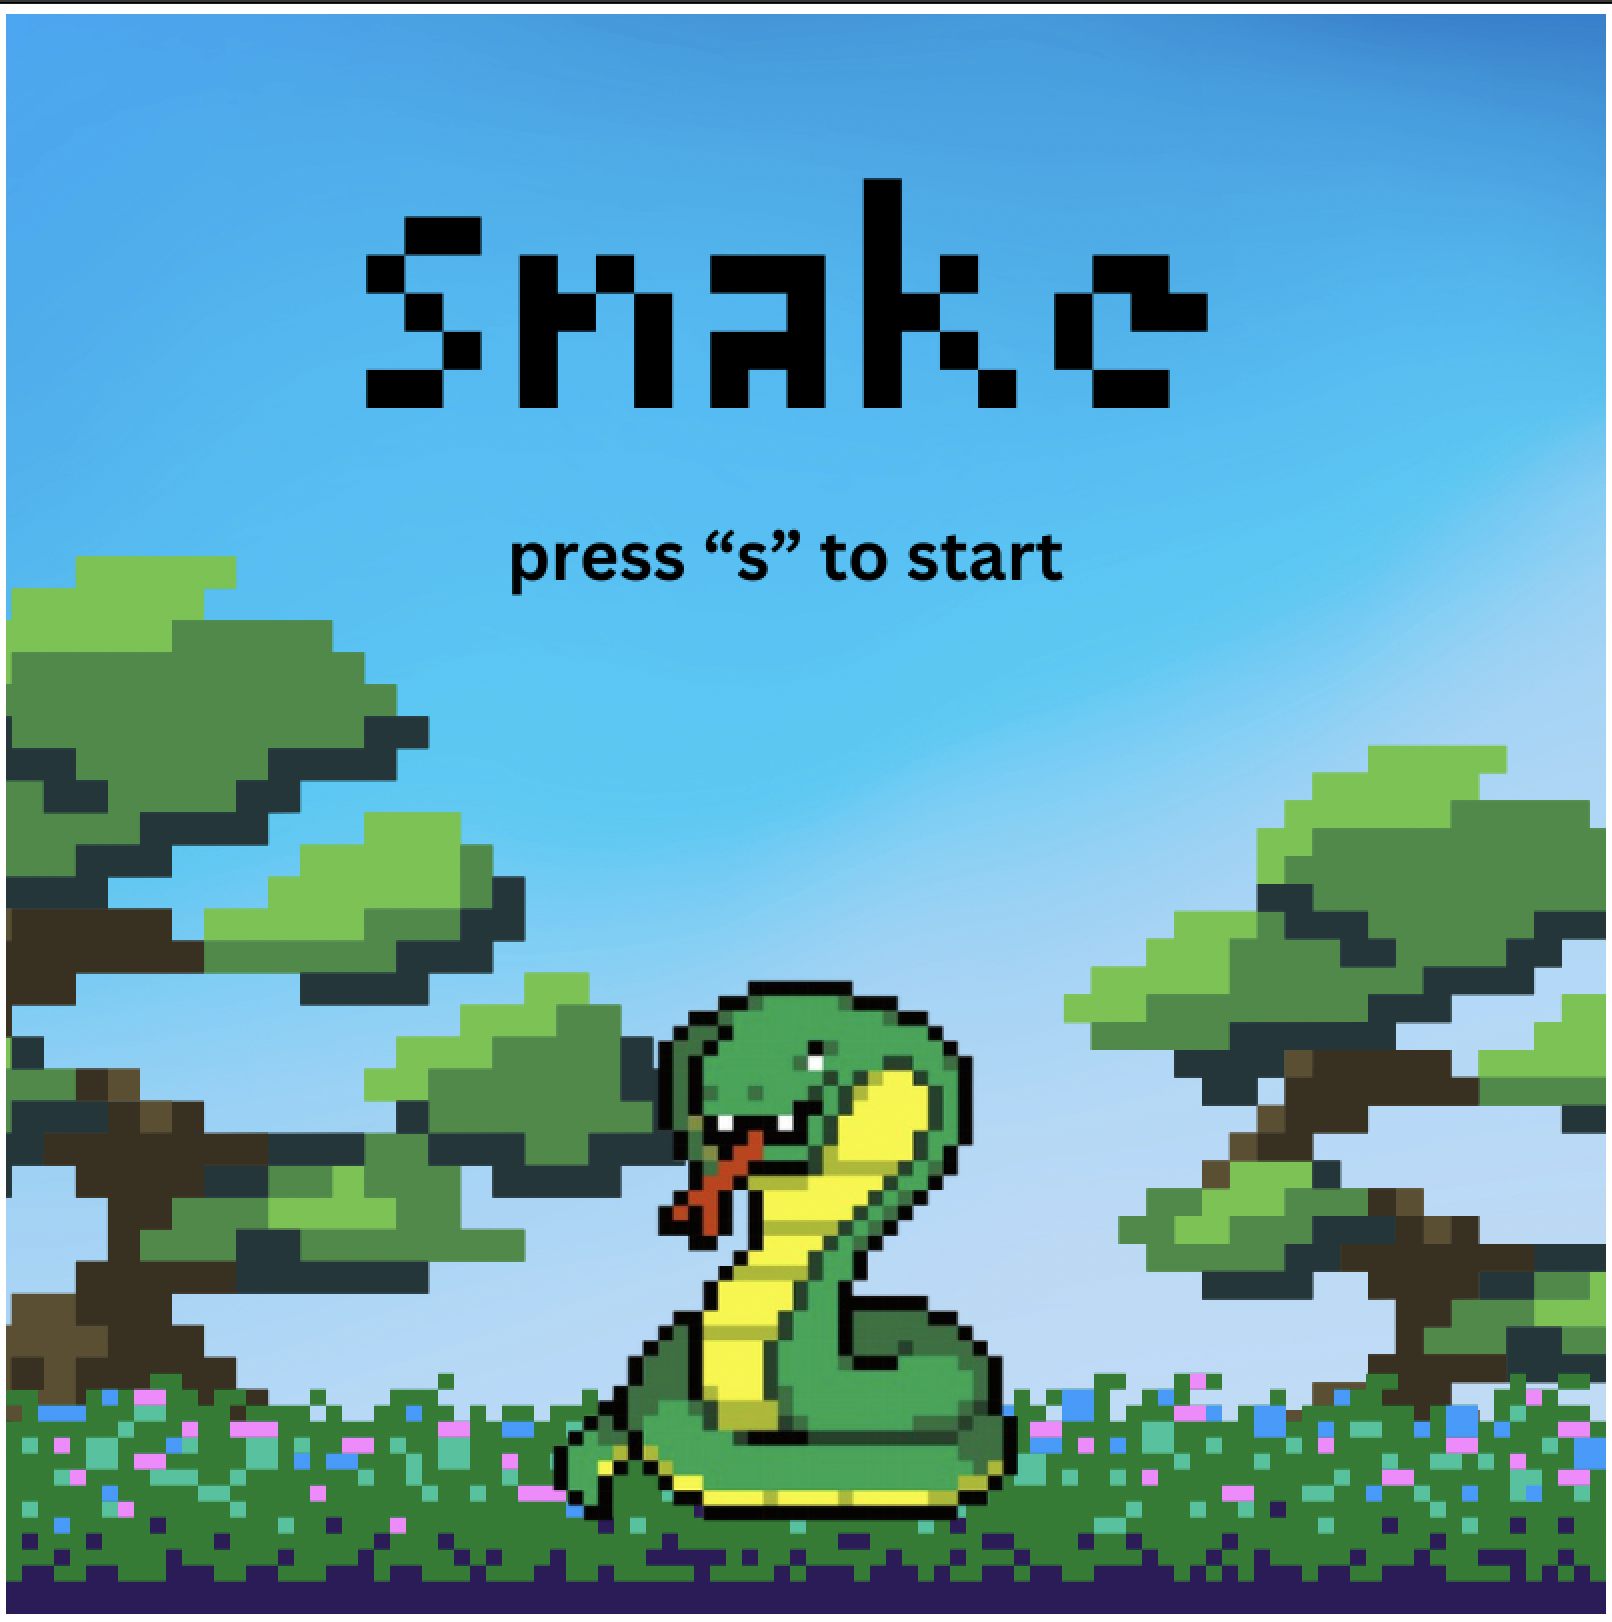
\includegraphics[width=.5\linewidth]{home.png}\\
		\Large{\textbf{Home Page}}
	\end{textblock*}
	
	\begin{textblock*}{10cm}(6cm,9cm)
		\centering
		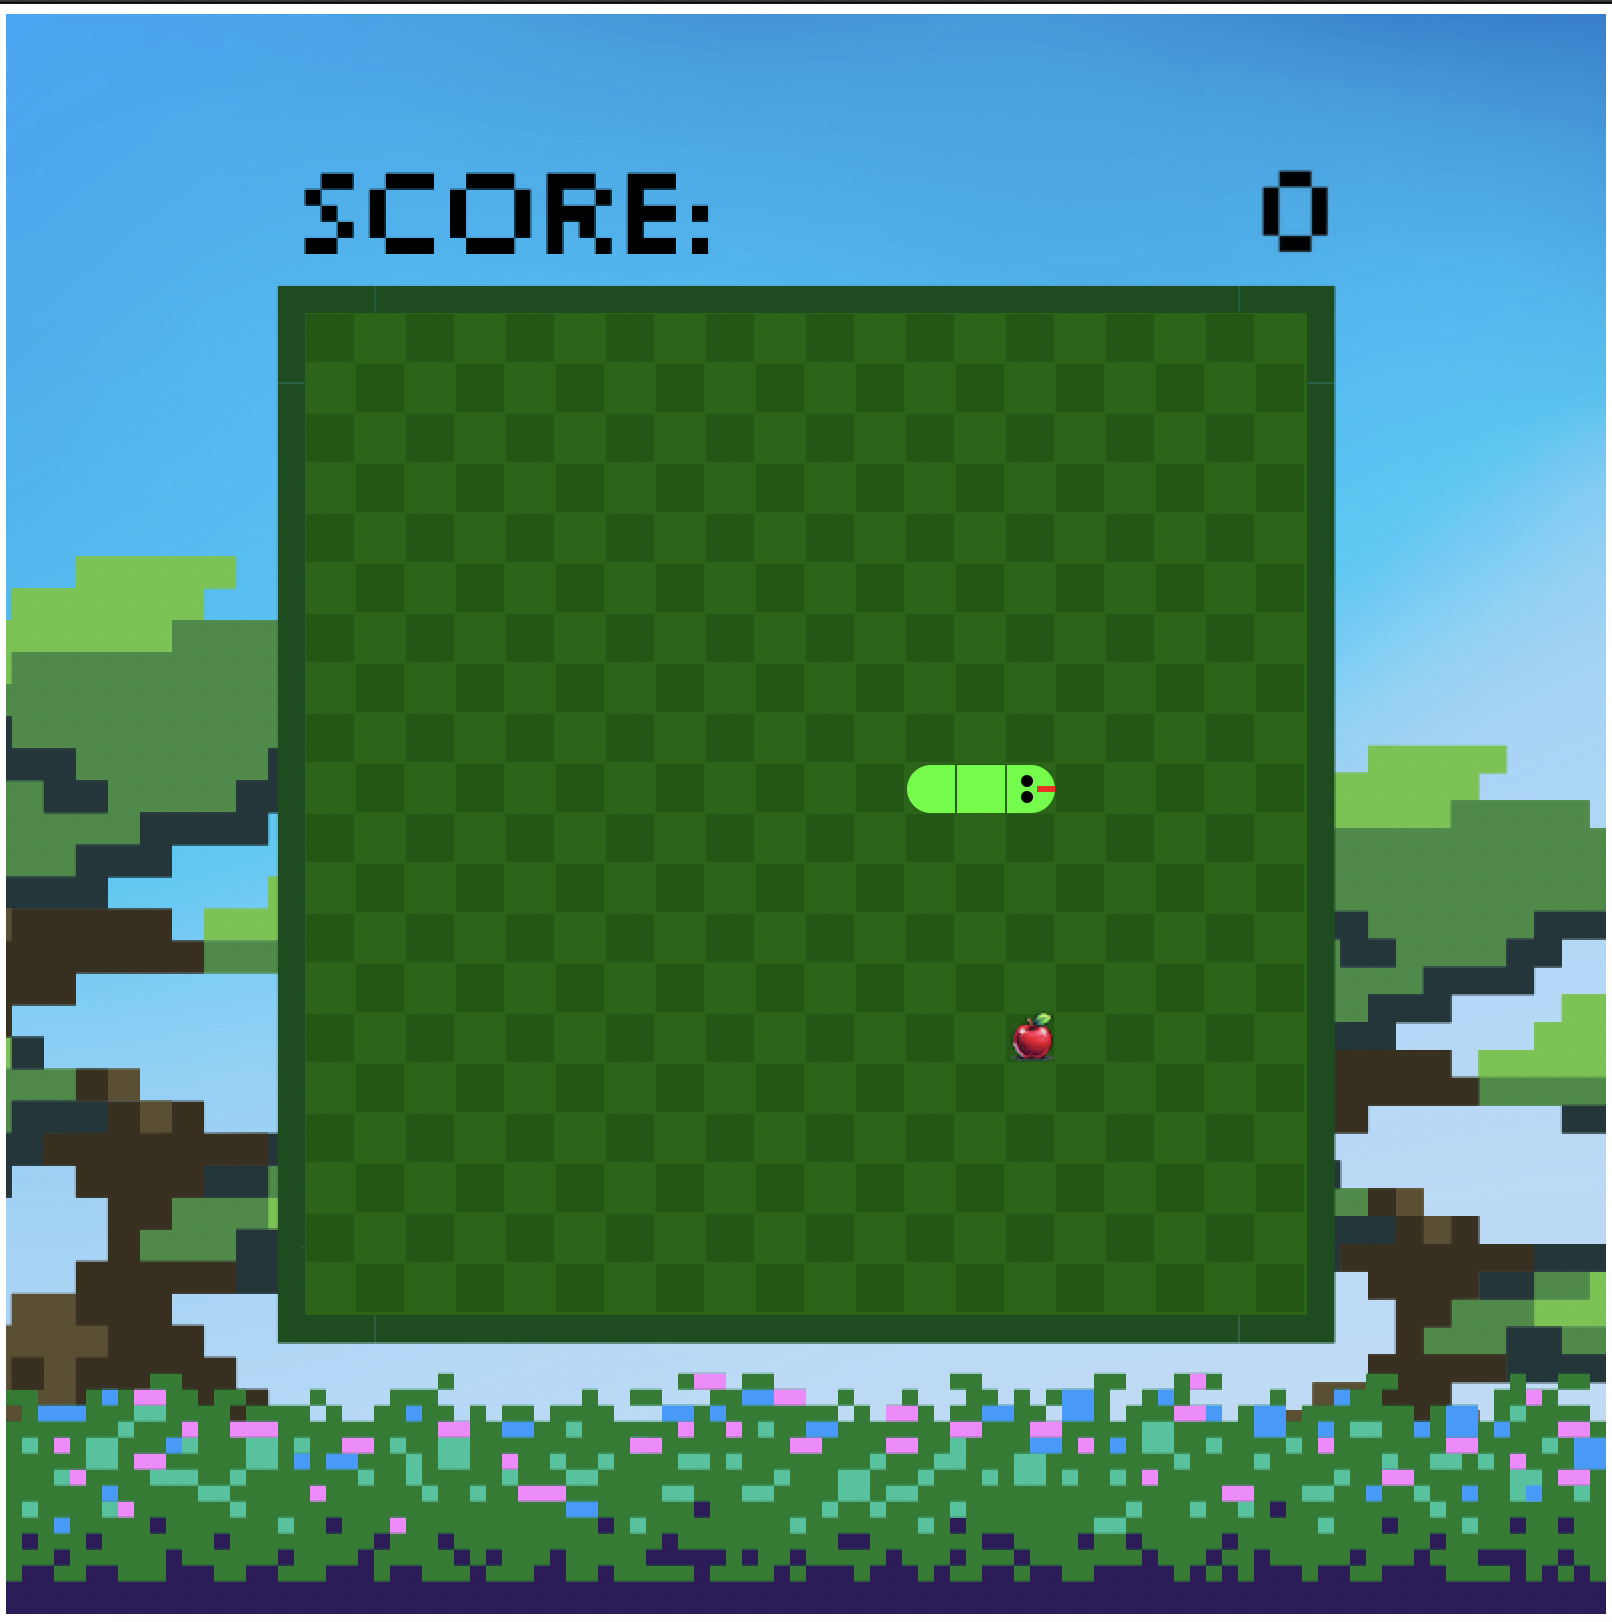
\includegraphics[width=.5\linewidth]{game.png}\\
		\Large{\textbf{Game}}
	\end{textblock*}
	
	\begin{textblock*}{10cm}(12cm,9cm)
		\centering
		
\includegraphics[width=.5\linewidth]{game-over.png}\\
		\Large{\textbf{Game Over}}
	\end{textblock*}
	
	\vspace{6.5cm}\section{Points}
	So, the aim of the game is to eat the most apple as possible, but, how do the points work and when does the snake's speed increase? Well, the score functioning is very simple: at the beginning of every game, the number of point is set to 0 by default and every time the snake eats an apple, it scores 100 points. There no limit, except for when there is no more space on the board.\\
	The speed of the snake does instead work very differently: we divided it into eight levels in order to start with a low speed and to finish with the highest one. However, the gamer is allowed and is encouraged to change and modify these levels of speed! In fact, if he wants to complicate the game by starting with a higher speed he can by modifying a game contant found on line 49 of the "snake-final.rkt " file. The constant to be modified is called RATE, and it can be setted to a positive integer value between 1 and 10. Beware: if the value is higher the snake will be too slow at the beginning.
	
\end{document}